\chapter{Bağıntılar ve Denklik}
\label{chap:bagintilar}


\par\smallskip{\sffamily\bfseries\color{cAcc}Öğrenme Hedefleri}\nopagebreak

\begin{itemize}\setlength{\itemsep}{2pt}\setlength{\parskip}{0pt}
\item İkili bağıntıyı ve temel özelliklerini (yansıma, simetri, geçişlilik) tanımlayabilme.
\item Denklik bağıntısı ile bölümleme arasındaki karşılıklılığı ispatlayabilme.
\end{itemize}

\section*{Bölüme Genel Bakış: İlişkiyi Matematikleştirmek}

‘Daha büyük’, ‘böler’, ‘denktir’, ‘bağlıdır’ — matematiğin ve gündelik dilin büyük bölümü ilişkiler üzerine kuruludur. Bir bağıntı (relation), bu sezgisel ‘ilişki’ fikrini kümeler diliyle kesinleştirir: A × A’nın bir alt kümesi. Charles Sanders Peirce ve Ernst Schröder on dokuzuncu yüzyılda bağıntıların cebirini geliştirdiler; Bourbaki geleneği ise bağıntıyı, fonksiyon dahil pek çok kavramın ortak zemini olarak matematiğin temeline yerleştirdi.

Bu bölüm iki bağıntı ailesine odaklanır: nesneleri ‘aynı sayan’ denklik bağıntıları ve nesneleri ‘sıralayan’ sıralama bağıntıları. İlki soyutlamanın (kesirler, mod sınıfları), ikincisi önceliklendirme ve yapının temelidir. Her ikisi de sonraki bölümlerde — kongrüanslar bir denklik, kardinalite karşılaştırması bir sıralama olarak — yeniden karşımıza çıkar. Böylece bağıntı kavramı, dersin teknik omurgasını birbirine bağlayan zemindir.

\section{Bağıntı ve Özellikleri}

\begin{tcolorbox}[bookbox,colback=cDef]\textbf{\textsf{\textcolor{cAcc}{Tanım.}}}\quad A üzerinde bir (ikili) bağıntı, R ⊆ A × A alt kümesidir; (a, b) ∈ R yerine a R b yazılır. R; yansımalı (her a için a R a), simetrik (a R b ⇒ b R a), ters simetrik (a R b ∧ b R a ⇒ a = b) veya geçişli (a R b ∧ b R c ⇒ a R c) olabilir.\end{tcolorbox}

\section{Denklik Bağıntısı}

Yansımalı, simetrik ve geçişli bir bağıntıya denklik bağıntısı denir. a elemanının denklik sınıfı [a] = \{x ∈ A: x R a\} biçiminde tanımlanır.

\begin{tcolorbox}[bookbox,colback=cDef]\textbf{\textsf{\textcolor{cAcc}{Teorem.}}}\quad Bir A kümesi üzerindeki denklik bağıntısının denklik sınıfları A’yı bir bölümlemeye (boştan farklı, ikişer ayrık, birleşimi A olan alt kümeler) ayırır; tersine, her bölümleme bir denklik bağıntısı tanımlar.\end{tcolorbox}

\begin{tcolorbox}[bookbox,colback=cEx]\textbf{\textsf{\textcolor{cAcc}{Örnek.}}}\quad İspat fikri (sınıflar örtüşmez): [a] ∩ [b] ≠ ∅ olsun; ortak bir c için c R a ve c R b. Simetri ve geçişlilikle a R b, buradan [a] = [b] gösterilir. Ayrıca her a ∈ [a] olduğundan sınıfların birleşimi A’dır. ∎\end{tcolorbox}

\begin{tcolorbox}[bookbox,colback=cDep]\textbf{\textsf{\textcolor{cAcc}{Muhakeme/Felsefe Derinleştirmesi — Sınıflandırma ve soyutlama bir muhakeme biçimi olarak}}}\quad Denklik bağıntısı, matematiğin en güçlü soyutlama araçlarından biridir: ‘aynı sayılacak’ nesneleri tek bir sınıfta toplar ve o sınıfı yeni bir nesne gibi ele almamızı sağlar (kesirler, mod-n sınıfları, yönler…). Bu, öğrencinin gündelik ‘gruplama’ sezgisinden biçimsel soyutlamaya geçişidir ve bir sonraki bölümde kongrüanslarda doğrudan iş görür.\end{tcolorbox}

\section{İleri Örnekler: Denklik, Bölüm Kümesi ve Sıralama}

Bağıntı özelliklerini tanımaktan, onlarla yapı kurmaya geçelim. Aşağıdaki örnekler denklik sınıflarının nasıl yeni nesneler ürettiğini ve sıralama bağıntılarının denklikten nasıl ayrıldığını gösterir.

\begin{tcolorbox}[bookbox,colback=cEx]\textbf{\textsf{\textcolor{cAcc}{Örnek.}}}\quad \textbf{Bölüm kümesi. }ℤ üzerinde a \textasciitilde{} b ⇔ 3 | (a − b) bağıntısı bir denkliktir. Üç denklik sınıfı vardır: [0] = \{…, −3, 0, 3, …\}, [1] = \{…, −2, 1, 4, …\}, [2] = \{…, −1, 2, 5, …\}. Bu sınıfların kümesi ℤ/\textasciitilde{} = \{[0], [1], [2]\} tam olarak ℤ₃’tür. Böylece bir denklik bağıntısı, sonsuz ℤ’den sonlu ve işlem yapılabilir yeni bir nesne üretir.\end{tcolorbox}

\begin{tcolorbox}[bookbox,colback=cEx]\textbf{\textsf{\textcolor{cAcc}{Örnek.}}}\quad \textbf{Kısmi sıralama. }ℕ⁺ üzerinde ‘a, b’yi böler’ (a | b) bağıntısı yansımalı (a | a), ters simetrik (a | b ∧ b | a ⇒ a = b) ve geçişlidir; yani bir kısmi sıralamadır. Ancak tam sıralama değildir: 2 ve 3 birbirini bölmediğinden karşılaştırılamazlar. Bu bağıntının Hasse diyagramında 1 en alttadır, asallar onun hemen üstünde yer alır ve her sayı, bölenlerinin üstüne çizilir.\end{tcolorbox}

\begin{tcolorbox}[bookbox,colback=cEx]\textbf{\textsf{\textcolor{cAcc}{Örnek.}}}\quad \textbf{Kapsama sıralaması. }Bir U kümesinin alt kümeleri üzerinde ‘⊆’ bir kısmi sıralamadır (yansıma, ters simetri, geçişlilik). ∅ en küçük, U en büyük elemandır; ancak iki ayrık küme karşılaştırılamaz olduğundan sıralama tam değildir.\end{tcolorbox}

\begin{tcolorbox}[bookbox,colback=cEx]\textbf{\textsf{\textcolor{cAcc}{Örnek.}}}\quad \textbf{Denklik olmayan bağıntı. }‘x, y ile arkadaştır’ bağıntısı simetriktir ama genelde geçişli değildir (arkadaşımın arkadaşı benim arkadaşım olmayabilir); dolayısıyla bir denklik bağıntısı değildir. Bu, üç özelliğin birbirinden bağımsız olduğunu hatırlatır.\end{tcolorbox}

\begin{tcolorbox}[bookbox,colback=cMis]\textbf{\textsf{\textcolor{cAcc}{Yaygın Kavram Yanılgıları}}}\quad \textbf{“Simetri ve geçişlilik, yansımayı da verir.” — }Yanlış. Bir eleman hiçbir şeyle ilişkili değilse (ör. boş bağıntı), simetri ve geçişlilik sağlansa bile yansıma sağlanmaz.\par\medskip{}\textbf{“Denklik sınıfları örtüşebilir.” — }İki sınıf ya tümüyle özdeştir ya da hiç kesişmez; kısmi örtüşme olamaz.\par\medskip{}\textbf{“Her sıralama tamdır (her iki eleman karşılaştırılabilir).” — }Kısmi sıralamada bazı elemanlar karşılaştırılamaz (2 ve 3, bölme sıralamasında).\par\medskip{}\textbf{“a R b ise her zaman b R a’dır.” — }Bu yalnızca simetrik bağıntılar için doğrudur; sıralamalar simetrik değildir.\par\medskip{}\textbf{“En büyük eleman ile maksimal eleman aynıdır.” — }En büyük eleman herkesten büyüktür; maksimal eleman yalnızca ‘üstünde başka eleman olmayan’dır. Kısmi sıralamada maksimal eleman birden çok olabilir, en büyük eleman ise en fazla bir tanedir.\end{tcolorbox}

\begin{figure}[htbp]
\centering
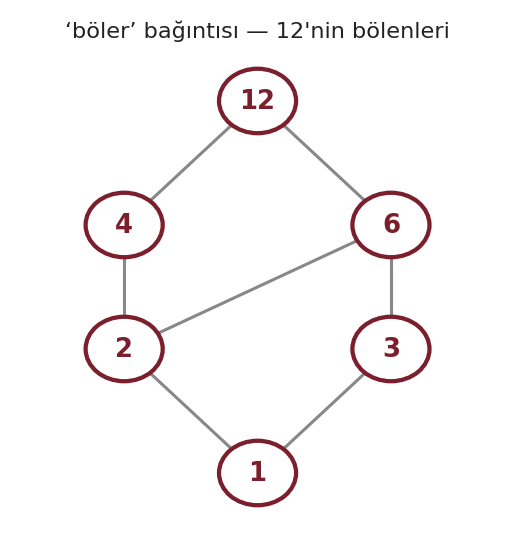
\includegraphics[width=0.56\linewidth]{figs/hasse.png}
\caption{12’nin bölenleri üzerinde ‘böler’ bağıntısının Hasse diyagramı.}
\end{figure}

\section{Uygulama ve Eğitime Yansıma}

Denklik bağıntısı, matematiğin ‘aynı kabul etme’ mekanizmasıdır ve her düzeyde iş görür: kesirler aslında ℤ × ℤ* üzerinde (a, b) \textasciitilde{} (c, d) ⇔ ad = bc denkliğinin sınıflarıdır (1/2 = 2/4 tam da bu yüzden); saat aritmetiği, yönler, geometrik benzerlik hep denklik sınıflarıdır. Öğrenciye ‘eşit olmadıkları hâlde aynı sayılan’ nesneleri fark ettirmek, soyutlamanın ilk ve en önemli adımıdır.

Sıralama bağıntıları ise önceliklendirme, çizelgeleme ve veri sıralama gibi uygulamaların temelidir. Öğretmen, ‘karşılaştırılamaz’ ögelerin bulunabileceği kısmi sıralamaları (ör. görevler arası bağımlılık) somut örneklerle göstererek, öğrencinin ‘her şey bir doğru üzerinde sıralanır’ önyargısını kırabilir.

\section{Yüksek Lisans Derinleştirmesi: Bölüm Kümesi, İyi Tanımlılık ve Sıralama Yapıları}

Bir denklik bağıntısı \textasciitilde{} verildiğinde, A/\textasciitilde{} bölüm kümesi ve π: A → A/\textasciitilde{}, π(a) = [a] kanonik izdüşümü ortaya çıkar. Matematiğin büyük bölümü bu inşa üzerine kuruludur: tam sayılardan rasyonellere, gruplardan bölüm gruplarına, topolojik uzaylardan bölüm uzaylarına. Bu geçişlerde kritik kavram ‘iyi tanımlılık’tır: A/\textasciitilde{} üzerinde bir işlem tanımlarken, sınıf temsilcisinden bağımsız olduğunu göstermek gerekir. Örneğin ℤₙ’de [a] + [b] = [a + b] tanımı ancak kongrüansın toplama ile uyumu (Bölüm~\ref{chap:kongruanslar}) sayesinde iyi tanımlıdır.

Sıralama yapıları da kendi zengin kavramlarını getirir. Bir kısmi sıralamada zincir (ikişer karşılaştırılabilir elemanlar) ve antizincir (ikişer karşılaştırılamaz elemanlar) ayrımı, en büyük/en küçük ile maksimal/minimal ayrımı ve üst/alt sınır kavramları, ileri matematikte (kafes kuramı, Zorn önsavı) merkezî rol oynar. İki sıralı kümenin ‘aynı biçimde sıralandığını’ söylemek için sıralama-koruyan bir eşleme (sıralama izomorfizmi) aranır; bu, Bölüm~\ref{chap:fonksiyonlar}’teki fonksiyon ve Bölüm~\ref{chap:kardinalite}’teki kardinalite fikirlerinin sıralama diline taşınmış hâlidir.

Böylece bağıntılar, dersin geri kalanını birbirine bağlayan zemindir: fonksiyon özel bir bağıntıdır (Bölüm~\ref{chap:fonksiyonlar}), kongrüans bir denkliktir (Bölüm~\ref{chap:kongruanslar}) ve kardinalite karşılaştırması bir tür sıralamadır (Bölüm~\ref{chap:kardinalite}). Bağıntı kavramını sağlam kurmak, bu üç bölümü ortak bir çatı altında görmeyi sağlar.

\section{Bağıntı İşlemleri: Bileşke, Ters ve Kapanış}

Bağıntılar da fonksiyonlar gibi birleştirilebilir ve dönüştürülebilir. Bir R ⊆ A × B ile S ⊆ B × C için bileşke S ∘ R = \{(a, c): ∃b, (a, b) ∈ R ∧ (b, c) ∈ S\} biçiminde tanımlanır. Ters bağıntı ise R⁻¹ = \{(b, a): (a, b) ∈ R\}. Bu işlemler, ilişkileri zincirlemeyi ve yönünü tersine çevirmeyi olanaklı kılar.

\begin{tcolorbox}[bookbox,colback=cEx]\textbf{\textsf{\textcolor{cAcc}{Örnek.}}}\quad \textbf{Bileşke. }R = ‘ebeveynidir’ ve S = ‘ebeveynidir’ ise S ∘ R = ‘büyükebeveynidir’. Bağıntı bileşkesi, ‘iki adımlık ilişkiyi’ tek bir bağıntı olarak ifade eder.\end{tcolorbox}

Bir bağıntı istenen bir özelliği sağlamıyorsa, onu sağlayan ‘en küçük’ genişlemesi aranabilir; buna kapanış (closure) denir. Yansımalı kapanış eksik olan (a, a) çiftlerini ekler; geçişli kapanış ise dolaylı olarak bağlı tüm çiftleri ekler. Örneğin bir yol ağında ‘doğrudan bağlantı’ bağıntısının geçişli kapanışı ‘bir yolla ulaşılabilir’ bağıntısını verir — bu, bilgisayar biliminde ulaşılabilirlik hesaplarının tam karşılığıdır.

\begin{tcolorbox}[bookbox,colback=cEx]\textbf{\textsf{\textcolor{cAcc}{Örnek.}}}\quad \textbf{Geçişli kapanış. }A = \{1, 2, 3\} üzerinde R = \{(1,2), (2,3)\} bağıntısı geçişli değildir. Geçişli kapanışı R⁺ = \{(1,2), (2,3), (1,3)\}; dolaylı bağ (1,3) eklenir. Bir denklik bağıntısı üretmek istersek ayrıca yansıma ve simetri kapanışlarını da almamız gerekir.\end{tcolorbox}

\section{Sıralama Türleri: Kısmi, Tam ve İyi Sıralama}

Sıralama bağıntıları kendi içinde katmanlıdır. Bir kısmi sıralamada (yansıma, ters simetri, geçişlilik) bazı elemanlar karşılaştırılamaz olabilir. Eğer her iki eleman karşılaştırılabiliyorsa sıralama tamdır (doğrusaldır): ℝ üzerindeki ‘≤’ böyledir. Bir adım ötede, boştan farklı her alt kümenin bir en küçük elemanı varsa sıralama iyi sıralamadır.

Bu ayrımlar önemlidir: ℕ, ‘≤’ ile iyi sıralıdır (Bölüm~\ref{chap:tumevarim}’daki tümevarımın dayanağı budur), ama ℤ ve ℝ tam sıralı oldukları hâlde iyi sıralı değildir — negatif tam sayılar kümesinin en küçüğü yoktur, (0, 1) açık aralığının da. İyi sıralama, seçim aksiyomuyla birlikte matematiğin derin sonuçlarına (her kümenin iyi sıralanabileceği, Zorn önsavı) bağlanır. Böylece Bölüm~\ref{chap:bagintilar}, sıradan ‘büyüklük karşılaştırması’ndan başlayıp modern matematiğin temel yapı taşlarına uzanan bir yelpazeyi kapsar; bu yapılar Bölüm~\ref{chap:fonksiyonlar}’teki fonksiyon ve Bölüm~\ref{chap:kardinalite}’teki kardinalite dilinde yeniden iş görür.

\section{Denklik Sınıflarıyla İnşa: Sayı Sistemleri}

Denklik bağıntısının matematikteki en güçlü uygulamalarından biri, yeni sayı sistemlerini eski olanlardan ‘kurmasıdır’. Bu inşalar, kesirlerin ve negatif sayıların aslında birer denklik sınıfı olduğunu ortaya koyar ve öğrencinin ‘sayı’ kavramına bakışını kökten değiştirir.

Tam sayıları doğal sayılardan kurmak için ℕ × ℕ üzerinde (a, b) \textasciitilde{} (c, d) ⇔ a + d = b + c bağıntısını tanımlarız. Buradaki sezgi, (a, b) çiftinin ‘a − b farkını’ temsil etmesidir; a + d = b + c koşulu, kesme (çıkarma) yapmadan ‘iki farkın eşitliğini’ yalnızca toplama diliyle ifade eder. Bu bağıntı bir denkliktir ve sınıfları tam sayıları verir: örneğin [(3, 5)] ile [(0, 2)] aynı sınıftır ve her ikisi de −2 tam sayısına karşılık gelir. Toplama ve çarpma, temsilcilerden bağımsız (iyi tanımlı) biçimde bu sınıflar üzerine taşınır.

Aynı fikir rasyonel sayıları verir. ℤ × ℤ* (paydası sıfırdan farklı çiftler) üzerinde (a, b) \textasciitilde{} (c, d) ⇔ ad = bc bağıntısı bir denkliktir ve sınıfları kesirlerdir. Burada 1/2 = 2/4 eşitliğinin gerçek anlamı ortaya çıkar: (1, 2) ile (2, 4) aynı denklik sınıfının iki temsilcisidir, çünkü 1·4 = 2·2. Yani ‘kesir sadeleştirme’ dediğimiz şey, aslında aynı denklik sınıfının farklı temsilcileri arasında geçiş yapmaktır.

\begin{tcolorbox}[bookbox,colback=cEx]\textbf{\textsf{\textcolor{cAcc}{Örnek.}}}\quad \textbf{İyi tanımlılık neden gerekir? }ℚ’de toplama [(a, b)] + [(c, d)] = [(ad + bc, bd)] biçiminde tanımlanır. Bu tanımın anlamlı olması için, temsilci değiştirdiğimizde sonucun değişmemesi gerekir. Örneğin 1/2 yerine 2/4 kullanırsak toplam yine aynı sınıfı vermelidir; bunu doğrulamak, denklik koşulunun (ad = bc) işlemle uyumunu göstermektir. İşte bu ‘iyi tanımlılık’ kontrolü, bölüm kümeleriyle çalışmanın değişmez bir parçasıdır.\end{tcolorbox}

Bu inşalar pedagojik olarak da aydınlatıcıdır. Öğrenciler çoğu zaman negatif sayıları ve kesirleri ‘gökten inmiş’ nesneler olarak öğrenir; oysa denklik sınıfı bakışı, bunların doğal sayılardan sistemli biçimde üretilebildiğini gösterir. Aynı desen ileride devam eder: gerçel sayılar rasyonellerin belirli dizilerinin denklik sınıflarıyla (Cauchy dizileri) kurulur. Böylece ‘denklik sınıfıyla inşa’, tek bir konu değil, matematiğin sayı sistemlerini büyütme yöntemidir.

Sonuç olarak Bölüm~\ref{chap:bagintilar}’in denklik bağıntısı, Bölüm~\ref{chap:kongruanslar}’nin kongrüans sınıflarıyla (ℤₙ) ve dersin sayı kavramına dair tüm tartışmasıyla derinden bağlantılıdır. Öğretmen adayı, ‘aynı kabul etme’nin biçimsel karşılığı olan denklik sınıfını kavradığında, hem soyut cebirin kapısını aralamış hem de okul matematiğindeki kesir ve tam sayı öğretimine çok daha derin bir zeminden bakabilir hâle gelmiş olur.

\begin{tcolorbox}[bookbox,colback=cDef]\textbf{\textsf{\textcolor{cAcc}{Tarihsel Not}}}\quad Bağıntıların matematiksel kuramı, on dokuzuncu yüzyılda Augustus De Morgan, Charles Sanders Peirce ve Ernst Schröder’in ‘bağıntı cebri’ çalışmalarıyla olgunlaştı. Aynı dönemde Richard Dedekind, gerçel sayıları rasyonellerin bir sıralama-bölünmesi (‘Dedekind kesitleri’) olarak tanımladı — sıralama bağıntısının, sayı sistemlerini kurmakta ne denli temel olduğunun çarpıcı bir örneği. Bugün bağıntı kavramı, veri tabanlarından graf kuramına kadar hesaplamalı matematiğin de ortak dilidir.\end{tcolorbox}

\section{Bağıntıları Görmek: Yönlü Graf ve Matris}

Sonlu bir küme üzerindeki bir bağıntı iki farklı biçimde ‘çizilebilir’: \emph{yönlü graf} olarak (her eleman bir nokta, her $(a,b)\in R$ çifti $a$’dan $b$’ye bir ok) ve \emph{bağıntı matrisi} olarak ($a$ satırı ile $b$ sütununun kesiştiği yere $(a,b)\in R$ ise 1, değilse 0). Bağıntının özellikleri bu iki temsilde gözle okunabilir; bu da soyut tanımları somut denetimlere dönüştürür.

\begin{figure}[htbp]
\centering
\begin{tikzpicture}[v/.style={circle,draw=acc,fill=accl,line width=.8pt,minimum size=7mm,font=\sffamily\small},>={Stealth[length=5pt]}]
\node[v] (1) at (0,1.6) {1}; \node[v] (2) at (1.8,1.6) {2};
\node[v] (3) at (0,0) {3}; \node[v] (4) at (1.8,0) {4};
\path[->,line width=.8pt,draw=bar] (1) edge[loop left,min distance=5mm] (1) (3) edge[loop left,min distance=5mm] (3) (2) edge[loop right,min distance=5mm] (2) (4) edge[loop right,min distance=5mm] (4);
\draw[->,line width=.8pt,bar] (1) to[bend left=18] (2); \draw[->,line width=.8pt,bar] (2) to[bend left=18] (1);
\draw[->,line width=.8pt,bar] (3) to[bend left=18] (4); \draw[->,line width=.8pt,bar] (4) to[bend left=18] (3);
\begin{scope}[on background layer]
\fill[grnl,rounded corners=8pt] (-.75,1.05) rectangle (2.55,2.2);
\fill[warml,rounded corners=8pt] (-.75,-.6) rectangle (2.55,.55);
\end{scope}
\node[anchor=west] at (3.6,.8) {$M_R=\begin{pmatrix}1&1&0&0\\1&1&0&0\\0&0&1&1\\0&0&1&1\end{pmatrix}$};
\node[small lbl,anchor=north] at (.9,-1.0) {yönlü graf};
\node[small lbl,anchor=north] at (5.1,-1.0) {bağıntı matrisi};
\end{tikzpicture}
\caption{$\{1,2,3,4\}$ üzerinde $R=\{(1,1),(2,2),(3,3),(4,4),$\allowbreak$(1,2),(2,1),(3,4),(4,3)\}$ bağıntısı. Her köşede döngü (yansıma), her ok çift yönlü (simetri); iki renkli bölge iki denklik sınıfıdır: $\{1,2\}$ ve $\{3,4\}$. Matriste sınıflar köşegen üzerindeki bloklar olarak görünür.}
\end{figure}

\begin{table}[htbp]
\centering\small
\renewcommand{\arraystretch}{1.3}
\begin{tabularx}{\linewidth}{>{\raggedright\arraybackslash}p{2.1cm}>{\raggedright\arraybackslash}X>{\raggedright\arraybackslash}X}
\toprule
\textbf{Özellik} & \textbf{Yönlü grafta} & \textbf{Matriste}\\
\midrule
Yansıma & Her noktada bir döngü vardır. & Köşegendeki bütün girdiler 1’dir.\\
Simetri & Her okun ters yönlüsü de vardır. & $M=M^{\mathsf T}$ (köşegene göre simetrik).\\
Ters simetri & Farklı iki nokta arasında en fazla bir yönde ok vardır. & $i\neq j$ için $m_{ij}$ ve $m_{ji}$ ikisi birden 1 olamaz.\\
Geçişlilik & $a\to b\to c$ yolu varsa $a\to c$ oku da vardır. & Boole çarpımı $M\odot M$’de 1 olan her yer $M$’de de 1’dir.\\
\bottomrule
\end{tabularx}
\caption{Bağıntı özelliklerinin iki temsilde okunması.}
\end{table}

\begin{ornek}[\textbf{Geçişli kapanış.}]
$\{1,2,3,4\}$ üzerinde $S=\{(1,2),(2,3),(3,4)\}$ bağıntısı geçişli değildir: $1\to2\to3$ yolu vardır ama $(1,3)\notin S$. $S$’yi kapsayan en küçük geçişli bağıntıyı (geçişli kapanış $S^+$) bulmak için, iki adımlı yollarla ulaşılabilen çiftleri ekleriz: $(1,3)$, $(2,4)$; ardından üç adımlı yolla $(1,4)$. Böylece
\[
S^+=\{(1,2),(2,3),(3,4),(1,3),(2,4),(1,4)\}
\]
olur. Grafta bu, ‘bir yol varsa doğrudan ok çiz’ kuralıdır. $S^+$ bir kesin sıralamanın ($<$) ta kendisidir: $a\,S^+\,b\iff a<b$.
\end{ornek}

\begin{ornek}[\textbf{Kaç bağıntı?}]
$n$ elemanlı bir küme üzerinde $n^2$ sıralı ikili, dolayısıyla $2^{n^2}$ bağıntı vardır. Yansımalı bağıntılarda köşegendeki $n$ girdi 1’e sabitlenir, kalan $n^2-n$ girdi serbesttir: $2^{n^2-n}$ yansımalı bağıntı. Simetrik bağıntılarda köşegen ($n$ girdi) ve köşegenin üstü ($n(n-1)/2$ girdi) serbestçe seçilir, altı buna göre belirlenir: $2^{n(n+1)/2}$ simetrik bağıntı. $n=3$ için bu sayılar sırasıyla $512$, $64$ ve $64$’tür. Matris temsili, sayma sorularını ‘hangi girdiler serbest?’ sorusuna çevirir.
\end{ornek}

\begin{yanilgi}[Kavram Yanılgısı — ‘Simetri ve geçişlilik yansımayı gerektirir’]
Yaygın bir ‘ispat’: ‘$a\sim b$ ise simetriden $b\sim a$; geçişlilikten $a\sim a$. O hâlde yansıma, öteki iki özellikten çıkar.’ Hata, her $a$ için \emph{bir} $b$ bulunduğunun sessizce varsayılmasıdır. $\{1,2\}$ üzerinde $R=\{(1,1)\}$ bağıntısı simetrik ve geçişlidir, ama $(2,2)\notin R$ olduğundan yansımalı değildir. Grafta: 2 numaralı nokta hiçbir okla bağlanmadığı için ‘ispattaki zincir’ hiç başlamaz. Bu örnek, ispatlarda niceleyici kapsamının (Bölüm~\ref{chap:niceleyiciler}) ne kadar önemli olduğunu gösterir.
\end{yanilgi}

\begin{sinif}[Sınıfta · Bağıntı kartları]
Gruplara dört elemanlı bir küme üzerinde farklı bağıntıların yönlü graflarını çizilmiş kartlar olarak verin. Her grup, kartları dört özelliğe göre sınıflasın ve her kararını graftaki bir ayrıntıyla (‘3 numaralı noktada döngü yok’) gerekçelendirsin. Ardından denklik bağıntısı olan kartlar için sınıfları renklendirip bir bölümleme yazdırın; ters yönde, verilen bir bölümlemeden bağıntının grafını kurdurun.
\end{sinif}

\section*{Alıştırmalar}

\reviewitem{1}{ℝ² üzerinde (a, b) \textasciitilde{} (c, d) ⇔ a² + b² = c² + d² bağıntısının bir denklik olduğunu gösterin ve denklik sınıflarını geometrik olarak betimleyin.}

\reviewitem{2}{\{1, 2, 3, 4, 6, 12\} kümesi üzerinde ‘böler’ bağıntısının Hasse diyagramını çizin.}

\reviewitem{3}{Bir küme üzerinde hem simetrik hem ters simetrik olan bir bağıntıya örnek verin ve neden ikisini birden sağladığını açıklayın.}

\reviewitem{4}{Bir denklik bağıntısının sınıflarının A’yı bir bölümlemeye ayırdığını (ikişer ayrık ve birleşimleri A) ispatlayın.}

\reviewitem{5}{ℤ üzerinde a \textasciitilde{} b ⇔ 5 | (a − b) bağıntısının tüm denklik sınıflarını yazın ve kaç tane olduğunu belirtin.}

\section*{Bölüm Özeti}

\begin{itemize}\setlength{\itemsep}{2pt}\setlength{\parskip}{0pt}
\item Bağıntı bir A × A alt kümesidir; yansıma, simetri, geçişlilik temel özelliklerdir.
\item Denklik bağıntısı ↔ bölümleme karşılıklılığı, soyutlamanın biçimsel temelidir.
\end{itemize}

\section*{Gözden Geçirme Soruları}

\reviewitem{1}{Tam sayılarda ‘a − b çifttir’ bağıntısının denklik bağıntısı olduğunu gösteriniz ve sınıflarını bulunuz.}

\reviewitem{2}{‘≤’ bağıntısı hangi özellikleri sağlar, hangilerini sağlamaz?}

\section*{Çoktan Seçmeli Sorular}

\mcqq{1}{Denklik bağıntısı hangi üç özelliği sağlar?}

\mcqo{A}{Yansıma, ters simetri, geçişlilik}

\mcqo{B}{Yansıma, simetri, geçişlilik}

\mcqo{C}{Simetri, geçişlilik, tamlık}

\mcqo{D}{Yansıma, simetri, tamlık}

\mcqa{B}{Denklik: yansıma, simetri, geçişlilik.}

\mcqq{2}{Denklik sınıfları A kümesini neye ayırır?}

\mcqo{A}{Bir sıralamaya}

\mcqo{B}{Bir bölümlemeye}

\mcqo{C}{Bir fonksiyona}

\mcqo{D}{Bir çarpıma}

\mcqa{B}{Denklik sınıfları kümeyi bir bölümlemeye ayırır.}

\mcqq{3}{İki denklik sınıfı [a], [b] için hangisi doğrudur?}

\mcqo{A}{Her zaman eşittir}

\mcqo{B}{Ya ayrıktır ya özdeştir}

\mcqo{C}{Her zaman ayrıktır}

\mcqo{D}{Kesişimleri tek elemanlıdır}

\mcqa{B}{İki sınıf ya tümüyle ayrıktır ya da özdeştir.}

\mcqq{4}{A üzerinde bir (ikili) bağıntı nedir?}

\mcqo{A}{A’nın alt kümesi}

\mcqo{B}{A × A’nın alt kümesi}

\mcqo{C}{A’dan A’ya fonksiyon}

\mcqo{D}{A’nın kuvvet kümesi}

\mcqa{B}{Bağıntı, A×A’nın bir alt kümesidir.}

\mcqq{5}{“Her a için a R a” özelliği hangisidir?}

\mcqo{A}{Yansıma}

\mcqo{B}{Simetri}

\mcqo{C}{Geçişlilik}

\mcqo{D}{Ters simetri}

\mcqa{A}{‘a R a’ yansıma özelliğidir.}

\mcqq{6}{“a R b ⇒ b R a” özelliği hangisidir?}

\mcqo{A}{Yansıma}

\mcqo{B}{Simetri}

\mcqo{C}{Geçişlilik}

\mcqo{D}{Ters simetri}

\mcqa{B}{‘aRb ⇒ bRa’ simetridir.}

\mcqq{7}{“a R b ∧ b R c ⇒ a R c” özelliği hangisidir?}

\mcqo{A}{Yansıma}

\mcqo{B}{Simetri}

\mcqo{C}{Geçişlilik}

\mcqo{D}{Ters simetri}

\mcqa{C}{Zincirleme geçiş, geçişlilik özelliğidir.}

\mcqq{8}{“a R b ∧ b R a ⇒ a = b” özelliği hangisidir?}

\mcqo{A}{Yansıma}

\mcqo{B}{Simetri}

\mcqo{C}{Geçişlilik}

\mcqo{D}{Ters simetri}

\mcqa{D}{‘aRb ∧ bRa ⇒ a=b’ ters simetridir.}

\mcqq{9}{a elemanının denklik sınıfı [a] nasıl tanımlanır?}

\mcqo{A}{\{x: x = a\}}

\mcqo{B}{\{x: x R a\}}

\mcqo{C}{\{a\}}

\mcqo{D}{∅}

\mcqa{B}{[a] = \{x: xRa\} biçiminde tanımlanır.}

\mcqq{10}{“≤” bağıntısı aşağıdaki özelliklerden hangisini sağlamaz?}

\mcqo{A}{Yansıma}

\mcqo{B}{Simetri}

\mcqo{C}{Geçişlilik}

\mcqo{D}{Ters simetri}

\mcqa{B}{‘≤’ ters simetriktir ama simetrik değildir.}

\mcqq{11}{Kongrüans (mod n) ℤ üzerinde ne tür bir bağıntıdır?}

\mcqo{A}{Sıralama}

\mcqo{B}{Denklik}

\mcqo{C}{Fonksiyon}

\mcqo{D}{Kısmi sıralama}

\mcqa{B}{Kongrüans yansıma/simetri/geçişlilik sağlar: denkliktir.}

\mcqq{12}{ℤ’de “a − b çifttir” bağıntısı nedir?}

\mcqo{A}{Denklik bağıntısıdır}

\mcqo{B}{Sıralamadır}

\mcqo{C}{Fonksiyondur}

\mcqo{D}{Hiçbiri}

\mcqa{A}{‘a−b çift’ bir denklik bağıntısıdır (parite).}

\mcqq{13}{Kısmi sıralama hangi üç özelliği sağlar?}

\mcqo{A}{Yansıma, simetri, geçişlilik}

\mcqo{B}{Yansıma, ters simetri, geçişlilik}

\mcqo{C}{Simetri, geçişlilik, tamlık}

\mcqo{D}{Yalnızca geçişlilik}

\mcqa{B}{Kısmi sıralama: yansıma, ters simetri, geçişlilik.}

\mcqq{14}{Bir bölümlemenin parçaları için hangisi doğrudur?}

\mcqo{A}{Örtüşürler}

\mcqo{B}{Boştan farklı, ikişer ayrık, birleşimleri A’dır}

\mcqo{C}{Tek elemanlıdırlar}

\mcqo{D}{A × A’yı verirler}

\mcqa{B}{Parçalar boştan farklı, ikişer ayrık, birleşimi A’dır.}

\mcqq{15}{Her bölümleme neyi tanımlar?}

\mcqo{A}{Bir fonksiyon}

\mcqo{B}{Bir denklik bağıntısı}

\mcqo{C}{Bir sıralama}

\mcqo{D}{Bir çarpım}

\mcqa{B}{Her bölümleme bir denklik bağıntısı belirler.}

\mcqq{16}{Denklik bağıntısı matematikte neden güçlü bir araçtır?}

\mcqo{A}{Sayma kolaylığı}

\mcqo{B}{Bir soyutlama aracı olarak ‘aynı sayılanları’ tek nesnede toplar}

\mcqo{C}{Görselleştirme}

\mcqo{D}{Hiçbiri}

\mcqa{B}{‘Aynı sayılanları’ tek nesnede toplayan bir soyutlama aracıdır.}

\mcqq{17}{A = \{1,2,3\} üzerinde R = \{(1,1),(2,2),(3,3)\} bağıntısı nedir?}

\mcqo{A}{Yalnızca simetriktir}

\mcqo{B}{Denklik bağıntısıdır (eşitlik bağıntısı)}

\mcqo{C}{Geçişsizdir}

\mcqo{D}{Ters simetrik değildir}

\mcqa{B}{Köşegen bağıntı tam olarak eşitliktir; bir denkliktir.}

\mcqq{18}{Bir denklik bağıntısının tüm sınıflarının birleşimi nedir?}

\mcqo{A}{Boş küme}

\mcqo{B}{Tüm A}

\mcqo{C}{Tek sınıf}

\mcqo{D}{A × A}

\mcqa{B}{Tüm sınıfların birleşimi kümenin tamamıdır.}

\mcqq{19}{“x ile y aynı doğum ayında” bağıntısı nedir?}

\mcqo{A}{Denklik bağıntısı}

\mcqo{B}{Sıralama}

\mcqo{C}{Fonksiyon}

\mcqo{D}{Ters simetri}

\mcqa{A}{‘Aynı doğum ayı’ yansıma/simetri/geçişlilik sağlar: denkliktir.}

\mcqq{20}{n denklik sınıfı olan bir bağıntı A’yı kaç parçaya böler?}

\mcqo{A}{n − 1}

\mcqo{B}{n}

\mcqo{C}{n + 1}

\mcqo{D}{2ⁿ}

\mcqa{B}{n sınıf, kümeyi n parçaya böler.}


\clearpage

\clearpage